The pinhole camera model is an ideal description of the mathematical relationship between the real 3D space and the 2D image projection. The pinhole camera is made up of a pinhole and an image plane. Because the pinhole is in between the image plane and the 3D world, any ray emitted from the 3D world has to pass through the pinhole before reaching the image plane. In this case the projected image is inverted.(\ref{fig:obscura}a) This natural phenomenon is called camera obscura and has been used through history being described by Ibn al-Haytham in the 10th century. If we place a plane in front of the pinhole, then the projected image won't be inverted.(\ref{fig:obscura}b) 

\begin{figure}[h]
    \centering
    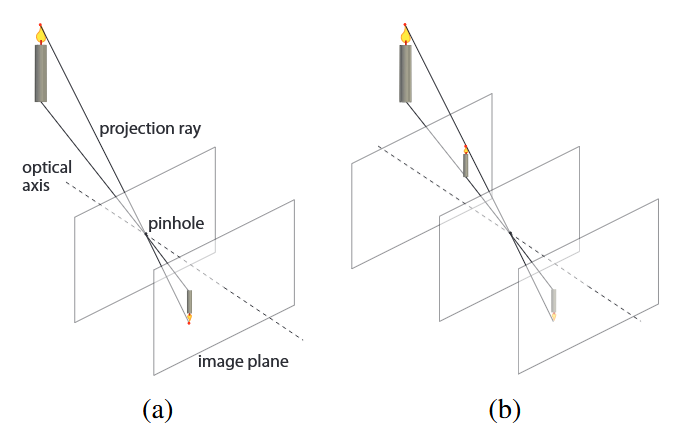
\includegraphics[width=0.5\linewidth]{imgs/obscura.png}
    \caption{Pinhole camera model}
    \label{fig:obscura}
\end{figure}

To mathematically understand this model, first we need to define 2 coordinate systems of interest. Those are:
\begin{itemize}
    \item The external coordinate system('W' for 'world') defined by center $\pmb{O_W}$ and axes $[X_W, Y_W, Z_W]$
    \item The camera coordinate system('C' for 'camera') defined by center $\pmb{O_C}$ and axes $[X_C, Y_C, Z_C]$
\end{itemize}



\begin{figure}[h]
    \centering
    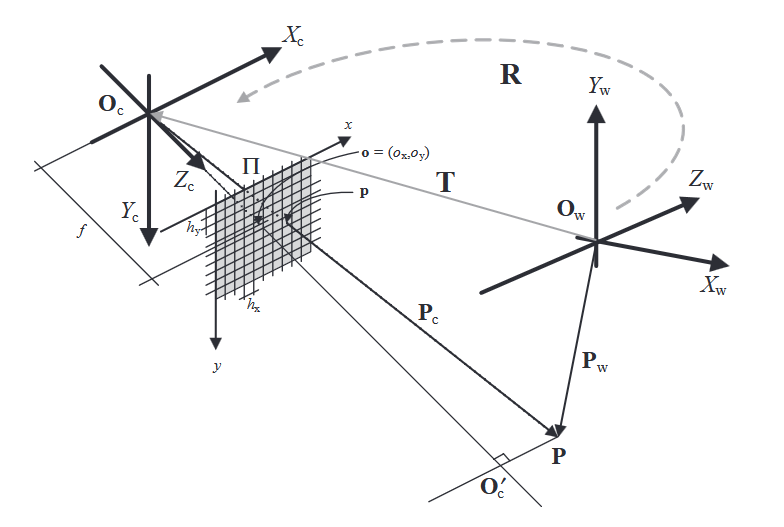
\includegraphics[width=0.8\linewidth]{imgs/pinholemodel.png}
    \caption{Pinhole camera model coordinate systems and points}
    \label{fig:pinhole}
\end{figure}

These 2 coordinate systems are related by translation $\pmb{T}$ and rotation $\pmb{R}$. \\
The following points can be seen on figure \ref{fig:pinhole}. \\
The image plane $\pmb{\Pi}$ is tessellated into rectangles called pixels. Pixels in a camera form discrete photosensing locations that sample any image projected onto the plane. Each pixel is indexed by a pair of coordinates expressed by natural numbers. $h_x$ and $h_y$ determine the physical dimensions of a single pixel. \\
Point $\pmb{O_C}$ called the focal point. Its projection onto $\pmb{\Pi}$ in $Z_C$ direction determines the principal point $o$ on the image plane. The distance from focal point $\pmb{O_C}$ to the principal point $o$ is called the focal length $f$. $Z_C$ is also called the principal axis. $\pmb{O_C}$, $o$ and $\pmb{O_C'}$ lie on it.  \\
We can define some point $\pmb{P}$ in the real world and its position is given by the chosen coordinate system, $\pmb{P_C}$ for the camera coordinate system or $\pmb{P_W}$ for the external coordinate system. \\
Point $\pmb{p}$ is an image of point $\pmb{P}$ onto the image plane with a center point $\pmb{O_C}$. We can define their coordinates as: 
\[
    \pmb{P} = [X, Y, Z]^T  \qquad \pmb{p} = [x, y, z]^T
\]


Because we have similar triangles $\triangle\pmb{O_C p o}$ and $\triangle\pmb{O_C P O_C'}$ we obtain:
\[
    x=f\frac{X}{Z} \qquad y=f\frac{Y}{Z} \qquad z =f
\]
The pinhole camera model can be defined by 2 sets of parameters:
\begin{itemize}
    \item Extrinsic parameters
    \item Intrinsic parameters
\end{itemize}